% Preamble: \pgfplotsset{width=10cm,compat=1.18}
\documentclass{article}
\usepackage[a5paper]{geometry}
\usepackage{pgfplots}
\usepackage{pdflscape}
\usepackage[extreme]{savetrees}
\usepackage{xstring}
\pgfplotsset{compat=1.18}
\begin{document}

\thispagestyle{empty}
\begin{landscape}
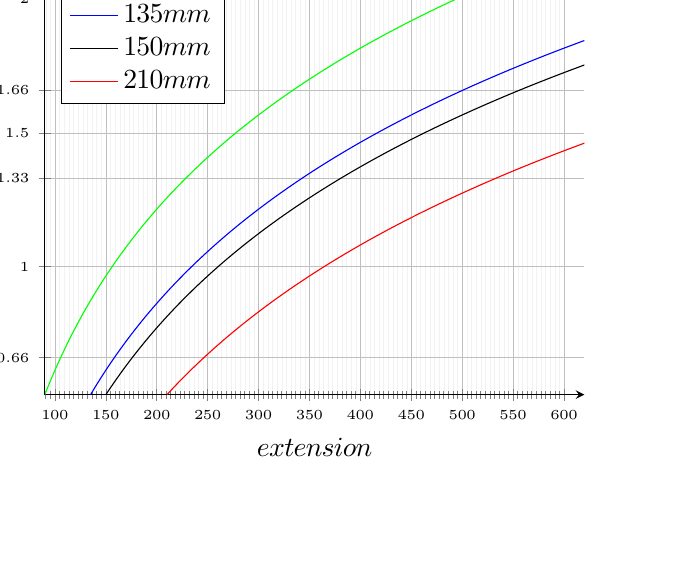
\begin{tikzpicture}
\centering
\usetikzlibrary{plotmarks}
\begin{axis}[
    axis lines = left,
    xlabel = \(extension\),
    ylabel = {\(stops\)},
    ticklabel style = {font=\tiny},
    xtick distance=50,
    minor x tick num=10,
    ytick={0.33,0.5,0.66,1,1.33,1.5,1.66,2.0,2.33,2.5,2.66,3},
    grid=both,
    grid style={line width=.1pt, draw=gray!10},
    major grid style={line width=.2pt,draw=gray!50},
    legend pos=north west,
]
\addplot [
    domain=90:620,
    samples=100,
    color=green,
]
{log10(((x / 90)^2) / log10(2)};
\addlegendentry{\(90mm\)}

\addplot [
    domain=135:620,
    samples=100,
    color=blue,
]
{log10(((x / 135)^2) / log10(2)};
\addlegendentry{\(135mm\)}

\addplot [
    domain=150:620,
    samples=100,
    color=black,
]
{log10(((x / 150)^2) / log10(2)};
\addlegendentry{\(150mm\)}

\addplot [
    domain=210:620,
    samples=100,
    color=red,
]
{log10(((x / 210)^2) / log10(2)};
\addlegendentry{\(210mm\)}

\end{axis}
\end{tikzpicture}
\end{landscape}

\thispagestyle{empty}
\begin{landscape}
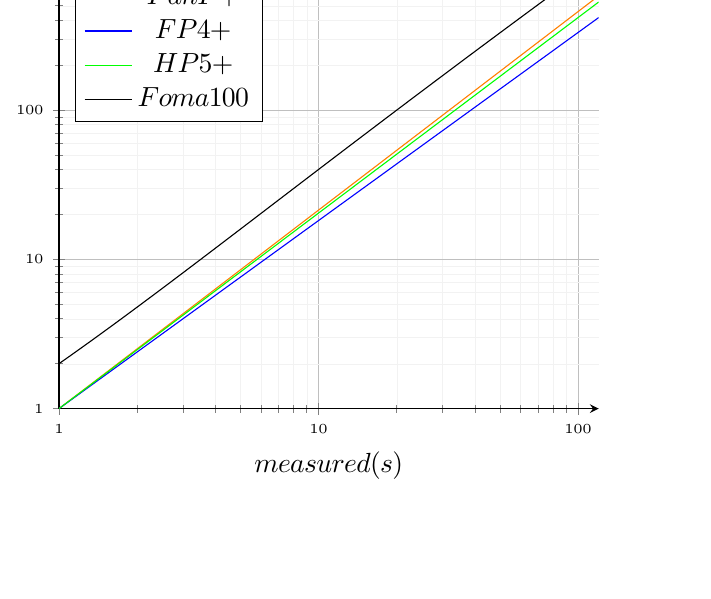
\begin{tikzpicture}
\centering
\usetikzlibrary{plotmarks}
\usepgfplotslibrary{units}
\begin{loglogaxis}[
    axis lines = left,
    xlabel = {\(measured(s)\)},
    ylabel = {\(actual(s)\)},
    ticklabel style = {font=\tiny},
    grid=both,
    grid style={line width=.1pt, draw=gray!10},
    major grid style={line width=.2pt,draw=gray!50},
    legend pos=north west,
    log ticks with fixed point,
]
\addplot [
    domain=1:120,
    samples=100,
    color=orange,
]
{x ^ 1.33};
\addlegendentry{\(PanF+\)}

\addplot [
    domain=1:120,
    samples=100,
    color=blue,
]
{x ^ 1.26};
\addlegendentry{\(FP4+\)}

\addplot [
    domain=1:120,
    samples=100,
    color=green,
]
{x ^ 1.31};
\addlegendentry{\(HP5+\)}

\addplot [
    domain=1:120,
    samples=100,
    color=black,
]
{(log10 x)^2 + (log10 x) + 2) * x};
\addlegendentry{\(Foma100\)}

\end{loglogaxis}
\end{tikzpicture}
\end{landscape}
\end{document}
